\begin{frame}{Konklusion}{Har vi flyttet noget?}
\section{Konklusion}
\begin{minipage}{0.6\textwidth}
\begin{block}{}
	\begin{itemize}
		\item \textbf{Et naturligt ønske:}\\ - Sikkerhed og virtuel fikstur
		\item \textbf{Opdelt løsningsstrategi:}\\ - Design og Analyse \\
		\scriptsize -\,\,\,\,Success i begge tilgange $\surd$ 
%		\vspace{0.5cm}
		\item \normalsize Sikkerhed \underline{kan} garanteres $\surd$
		\item Virtuel fikstur \underline{kan} opnås $\surd$
		\vspace{0.5cm}
		\item \normalsize ROS interface  $\surd$ \\
		\scriptsize - startet fra scratch (næsten) \\
		\scriptsize - velfungerende setup $\surd$ \\
\scriptsize - enhver real-time controller $\surd$ \\
		\item \normalsize En stejl læringskurve er brudt \\ 
		\scriptsize - der kan arbejdes videre på projektet
	\end{itemize}
\end{block}
\end{minipage}
\begin{minipage}{0.35\textwidth}

\includegraphics[width=1\linewidth]{blowing-a-dandelion-600.jpg}
\vspace*{0.2cm}


\includegraphics[width=1\linewidth]{TwoPaths-900x470.jpg}
\vspace*{0.2cm}

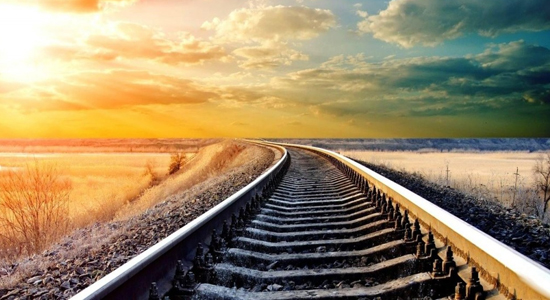
\includegraphics[width=1\linewidth]{path-to-success.jpg}
\end{minipage}
\end{frame}

\begin{frame}{Konklusion}{Konklusion på design tilgangen}
\begin{itemize}
	\item Relativt intuitiv designprocedure \\	\vspace*{0.08cm}
	\scriptsize {\color{white}{m}} 1. Lav model \\	
    \scriptsize {\color{white}{m}} 2. Konstruer CBF udfra fysiske forhold og beregn Lie afledede\\	
    \scriptsize {\color{white}{m}} 3. Specificer $\epsilon$ sådan at $\mathcal{T}$ er "tilpas" \\	
    \scriptsize {\color{white}{m}} 4. Design en vilkårlig controller i det sikre område \\ 	
    \scriptsize {\color{white}{m}} 5. Kombiner "sikker" og "usikker" controller \\
	\item \normalsize Kreativitet er nødvendigt når en CBF skal konstrueres
	\item Brug når der er et fysisk forhold til tilstandene
	\item Brugbar og effektiv (ikke beregningstung)
\end{itemize}
\vspace*{0.2cm}

\includegraphics[width=0.245\linewidth]{checklist.jpg} \hspace*{0.2cm}

\includegraphics[width=0.32\linewidth]{p01tgd39.jpg} \hspace*{0.2cm}
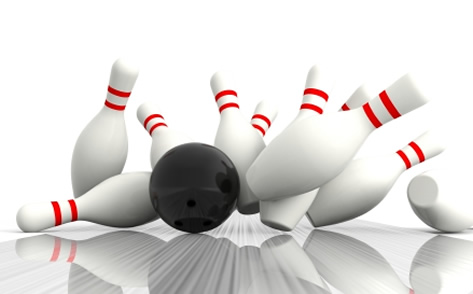
\includegraphics[width=0.34\linewidth]{Effective-design1.jpg}
\end{frame}



\begin{frame}{Konklusion}{konklusion på analyse tilgangen}
\begin{itemize}
%	\item Global (SOS) til lokal (Putinars Positivstellensatz)
	\item Et framework er udviklet
\end{itemize}

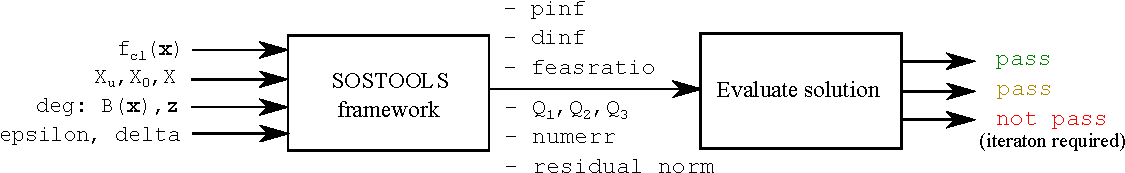
\includegraphics[width=1\linewidth]{sostools_eval.pdf}

\begin{itemize}
	\item Kan nemt udvides til flere dimensioner
%	\item \textbf{Budskab:} Når en grøn løsning er fundet - Stop
%	\item \textbf{Anvendelse:} Forstå betydningen af $\Delta, \epsilon, g_j$ og $deg$.
%	\item \textbf{Udvidelse i dimensioner:} Trivielt, men der skal defineres nye intervaller for \textit{g} polynomier 
	\item Abstrakt teori er analyseret, anvendt sammen med SOSTOOLS og en guide er udarbejdet
\end{itemize}
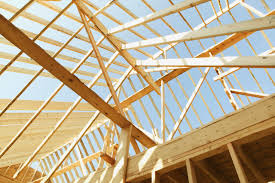
\includegraphics[width=0.31\linewidth]{imagesframe.jpg} \hspace*{0.5cm}

\includegraphics[width=0.21\linewidth]{Search.jpg} \hspace*{0.5cm}

\includegraphics[width=0.33\linewidth]{imagesabs.jpg} 
\end{frame}

\begin{frame}{Fremtidigt arbejde}{Vi er ikke stærkere end det svageste led i kæden}
\begin{minipage}{0.65\textwidth}
\begin{block}{}
	\begin{itemize}
		%\item Fejl-tolerant kontrol % \\ 
		%\scriptsize {\color{white}{m}} - Hvad hvis vi mister en sensor?
		\item \normalsize Kompleksitet af barrierefunktioner
		\item \normalsize Robust/fejl-tolerent kontrol %\\ 
%		\scriptsize {\color{white}{m}} - Modeller vil altid være forsimplet!
		\item \normalsize Inkorporere integralvirkning \\ 
%		\scriptsize {\color{white}{m}} - især tydeligt ved det dynamiske system
		\item \normalsize Synkronisering med hjerte
%		\item lave en tre delining i $\mathcal{T}$
		\item \normalsize End effector orientering \\
		\scriptsize {\color{white}{m}} -  Sikre sikkerhed for rammen
		\item \normalsize  Trajektorie planlægning \\ 
		\scriptsize {\color{white}{m}} - hvis springet mellem \textit{x} og \textit{x}$_{\text{ref}}$ er for stort
%		\item \normalsize Tachometer kan blive "forvirret"
		\item \normalsize Skræddersy IK solver
		\item Øge sampling rate til 2\,kHz \\
		\scriptsize {\color{white}{m}} - UDP i stedet for TCP/IP
		\item \normalsize  Monte Carlo simulering ved brug af SOSTOOLS framework
	\end{itemize}
\end{block}
\end{minipage}
\begin{minipage}{0.3\textwidth}
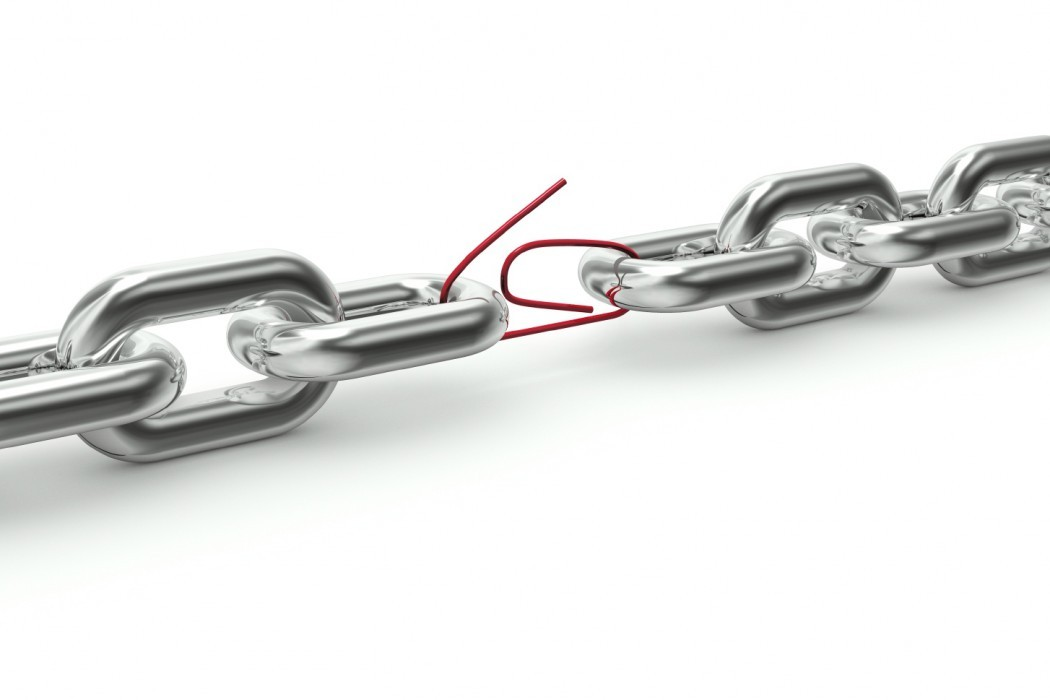
\includegraphics[width=1\linewidth]{The-Weak-Link-in-the-Chain-474557-2.jpg}
\vspace*{0.2cm}


\includegraphics[width=1\linewidth]{work_with_us.jpg}
\vspace*{0.2cm}

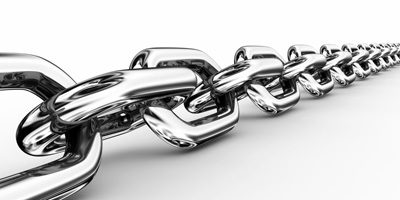
\includegraphics[width=1\linewidth]{chain-links-WEB.jpg}
\end{minipage}
\end{frame}